%%=============================================================================
%% Methodologie
%%=============================================================================

\chapter{\IfLanguageName{dutch}{Methodologie}{Methodology}}
\label{ch:methodologie}

%% TODO: Hoe ben je te werk gegaan? Verdeel je onderzoek in grote fasen, en
%% licht in elke fase toe welke stappen je gevolgd hebt. Verantwoord waarom je
%% op deze manier te werk gegaan bent. Je moet kunnen aantonen dat je de best
%% mogelijke manier toegepast hebt om een antwoord te vinden op de
%% onderzoeksvraag.
\section{Hoe de onderzoeksvraag tot stand is gekomen.}
\label{POC_introduction}
Dit onderzoek ontstond uit een persoonlijke interesse. Internet is een zeer veranderlijk geheel met tal van nieuwe technologieën die vervolgens ingeburgerd raken. Software ontwikkeling is dan ook geen vast gegeven. Toch zijn er een aantal basisfundamenten waarop softwareontwikkeling gebaseerd is. Een van deze fundamenten is het klassieke server-client model. In dit model voorziet één centrale computer bestanden of diensten voor tal van andere computers. Een gekend voorbeeld hiervan is de manier waarop het internet werkt ook wel bekend onder het HTTP protocol.\\

Bestaat er dan geen alternatief voor het Client-Server model? Distributed Computing tracht deze vraag te beantwoorden. Eén van de oplossingen is een zogenaamd P2P netwerk. Binnen dit type netwerk voorzien computers onderling bestanden en diensten aan elkaar. Dit type netwerk werd vooral populair onder de vorm van File-Sharing Protocollen. Gekende voorbeelden zijn hierbij Pirate Bay en Napster. Hoewel deze protocollen een eenvoudig en elegant alternatief boden, stonden ze nog niet op punt. Zo was er geen manier om op een veilig wijze aan dataopslag te doen.\\

Blockchain bracht een oplossing voor het probleem van dataopslag. Blockchain technologie is vooral bekend van Bitcoin en de financiële impact die deze met zich mee bracht. Toch zijn de implicaties veel diepgaander. Blockchain biedt een manier om op een veilige wijze aan dataopslag te doen in een gedistribueerd netwerk. Doordat data integriteit kan gewaarborgd worden kunnen ontwikkelaars veiligere en robuustere oplossingen ontwikkelen voor een P2P netwerk.\\

Toch bleef de blockchain technologie niet beperkt tot Bitcoin en P2P netwerken en werd ze veel verder ontwikkeld. Zo kwam Ethereum met het idee van smart contracts die software ontwikkelaars in staat stellen om transacties op Blockchain netwerken verder te controleren. Hierdoor kunnen applicaties worden ontwikkeld die op een volledig gedistribueerde manier werken. Het is een zeer fascinerende en revolutionaire manier van denken die grote implicaties met zich mee kan bregen.\\

Deze bachelorproef wil deze technologie verkennen en gebruiken in één van de meest fundamentele stappen van moderne software ontwikkeling: versiebeheer.\\

Uiteraard is deze bachelorproef niet het enige onderzoek over het decentraliseren van versiebeheer. In hun onderzoek decentraliseren \textcite{Nizamuddin2019} versiebeheer aan de hand van de Ethereum blockchain en IPFS. Dit is een zeer interessante benadering geweest maar te beperkt. Veel van de achterliggende concepten werden niet uitgelegd en hun oplossing was eerder beperkt in grootte in en complexiteit. Deze bachelorproef wilt hierop een aanvulling bieden en uitleggen wat blockchain, versiebeheer en IPFS exact zijn en hoe deze kunnen worden gecombineerd.

\section{Het ontleden van de onderzoeksvraag.}
\label{ontleden van de onderzoeksvraag}
Zoals besproken in \ref{POC_introduction} is de uiteindelijke onderzoeksvraag waarop een antwoord wordt gezocht: \textbf{Hoe kan men door middel van Blockchain principes en IPFS een werkbaar gedecentraliseerd versiebeheersysteem ontwikkelen?} Deze wordt onderverdeeld in verschillende deelvragen die sequentieel zijn beantwoord in de literatuurstudie. Hieronder volgt een kort overzicht en antwoord op de verschillende deelvragen. Voor meer informatie zie \ref{ch:stand-van-zaken}.
 
\begin{table}[h!]
\begin{tabularx}{\linewidth}{ |X|X| }
\hline
Deelvraag & Antwoord \\ \hline
Wat zijn de problemen die versiebeheersystemen oplossen? & 
Versiebeheersystemen bieden een manier om verschillende softwareversies aan te maken. Hierdoor kunnen softwareontwikkelaars ten allen tijden toegang krijgen tot verschillende versies van hun software. Versiebeheersystemen stellen ontwikkelaars in staat om hun code op een eenvoudige manier onderling met elkaar te delen en samen te werken.\\ \hline
Waaruit bestaat een versiebeheersysteem? & Een versiebeheersysteem bestaat uit twee delen: een manier om bestanden op te slaan en te delen met elkaar. Ten tweede een wijze om bestanden te archiveren. Dit wilt zeggen dat ze verschillende versies van de bestanden kunnen opslaan en ook toegang bieden tot deze versies.\\ \hline
Waarom zouden we van gecentraliseerde (server-client architectuur) versiebeheersystemen overstappen naar een gedecentraliseerde variant?         & Moderne versiebeheersystemen zijn vaak het eigendom van grote tech-giganten. Binnen software ontwikkeling streven open-source developers en bedrijven naar democratische softwareontwikkeling. Gedecentraliseerde systemen kaderen goed binnen deze ideologie. Gedecentraliseerde systemen hebben ook het voordeel dat ze geen centrale server architectuur vereisen. Servers zijn immers kostelijk en mocht de server kapot gaan is men alle gegevens kwijt (\textit{het zogenaamde SPOF probleem}).\\ \hline
Wat zijn de eigenschappen en valkuilen van gedecentraliseerde(P2P) netwerken? & P2P netwerken bieden een manier om op een gedecentraliseerde wijze diensten en software aan te bieden. Elke peer zal hierbij de rol van zowel server als client op zich nemen om dit te bereiken. Het grootste nadeel is echter dat deze netwerken een groot aantal deelnemers vereisen om functioneel werkbaar te zijn.\\ \hline
\end{tabularx}
\end{table} 
\newpage
\begin{table}[t!]
\begin{tabularx}{\linewidth}{ |X|X| }
\hline
Deelvraag & Antwoord \\ \hline
Wat is IPFS en hoe kadert het binnen versiebeheer? & IPFS is een P2P file-sharing protocol. Door IPFS kan men op een gedecentraliseerde wijze bestanden gaan opslaan en opvragen. Aangezien versiebeheersystemen toegang willen bieden tot het delen van software versies zijn daar uiteraard ook bestanden bij betrokken. Een softwareproject is immers niets meer of minder dan verschillende bestanden. Hiervoor is IPFS dus een geschikte kanidaat.\\ \hline
Wat zijn smartcontracts en hoe bieden ze een meerwaarde aan Blockchain applicaties? & Smartcontracts is een manier om op een gedecentraliseerde wijze code uit te voeren en de data in de blockchain aan te passen. Zo kan men voorwaarden opleggen aan wijzigingen in de data. Door smartcontracts kan men bijvoorbeeld enkel de eigenaar van bepaalde data toestaan om deze data te wijzigen.\\ \hline
\end{tabularx}
\end{table} 
\newpage
\newpage
Bovenstaande deelvragen bieden een goed overzicht van wat er exact nodig is om een Proof Of Concept op te stelen. De eigenlijke doelstelling van de onderzoeksvraag is het bekomen van een gedecentraliseerd versiebeheer systeem. Welke eigenschappen moet de POC voorzien om te voldoen aan deze vereisten?:

\begin{enumerate}
	\item De oplossing die wordt ontwikkeld mag geen centrale component hebben en moet op een volledig gedistribueerde manier in staat zijn om te functioneren.
	\item De oplossing moet een gebruiker in staat stellen om documenten met anderen te kunnen delen.
	\item De oplossing moet een manier aanbieden om wijzigingen aan deze documenten op te slaan onder de vorm van verschillende versies. Deze verschillende versies moeten kunnen geraadpleegd worden.
\end{enumerate}

\section{Tools}
\label{Tools}
Het delen van bestanden wordt mogelijk gemaakt door middel van IPFS. Dit protocol stelt de POC in staat om bestanden te verspreiden op een gedistribueerde manier en deze vervolgens opnieuw op te vragen. Hiervoor gebruikt IPFS het principe van een CID. Dit is in essentie een zelfbeschrijvende hash code die vervolgens kan worden gebruikt om bestanden op te halen -zie \ref{ipfs_decent}-. IPFS stelt ons ook in staat om meerdere versies van dezelfde bestand(en) op te slaan en ter beschikking te stellen. Neem bijvoorbeeld onderstaand scenario:\\

Bob en Alice willen een website ontwikkelen. Bob plaatst de homepagina op het IPFS netwerk en krijgt een CID om dit bestand opnieuw op te vragen. Hij deelt deze CID met Alice die vervolgens het bestand lokaal binnenhaalt. Alice brengt enkele wijzigingen aan en zet het bestand opnieuw op het netwerk. Alice zal een nieuwe CID worden toegewezen. Er zijn nu in feite twee verschillende versies van dit bestand op het netwerk, een versie van Bob die kan worden opgehaald met de CID die Bob heeft en een versie van Alice met haar eigen CID.\\

Toch is IPFS op zich niet voldoende. Er is immers geen eenvoudige manier voorzien om deze CIDS met elkaar te delen. Hier biedt blockchain een oplossing. Blockchain functioneert immers als een databank. De CIDS kunnen daar dus worden bewaard en opgevraagd. Om dit proces van opslaan en opvragen te vereenvoudigen wordt gebruik gemaakt van smart contracts. Niet iedere blockchain ondersteunt deze smartcontracs. Ethereum is een gekend voorbeeld van een netwerk dat dit wel ondersteunt.\\

Deze smartcontracts worden geschreven in de programmeertaal Solidity. Veel netwerken vragen transactiekosten voor het werken met smartcontracts . Om deze transactie kosten te vermijden kan er gebruik gemaakt worden van een lokaal Ethereum netwerk. Dit lokaal netwerk voorziet dezelfde functies maar heeft geen transactiekosten. De software die hiervoor gebruik wordt is \textcite{Ganache}.\\

Het ontwikkelen en testen van smartcontracts is ook niet evident. Om dit te vergemakkelijken wordt gebruik gemaakt van de \textcite{Truffle}. Deze suite biedt de mogelijkheid om smartcontracts te testen. Hiervoor wordt gebruik gemaakt van het javascript framework Mocha.js. Truffle wordt ook gebruikt om de smartcontracts die worden ontwikkeld op de lokale blockchain uit te rollen.\\

Tot slot wordt er gebruik gemaakt van een console applicatie geschreven in Dotnet-core 3.1 om de verschillende elementen samen te brengen. Deze console applicatie zal onder andere de verschillende bestanden op het IPFS netwerk plaatsen en de smartcontracts op de blockchain aanspreken. Om smartcontracts te kunnen aanspreken vanuit onze console applicatie zal gebruik gemaakt worden van \textcite{Nethereum}. Om IPFS te kunnen gebruiken wordt gebruik gemaakt van \textcite{IPFSClient}.\\

\section{Meetbare criteria}
Zoals hierboven vermeld wordt -zie \ref{ontleden van de onderzoeksvraag} zijn er drie eigenschappen waaraan het ontwikkelde prototype moet voldoen:

\begin{enumerate}
	\item De oplossing die wordt ontwikkeld mag geen centrale component hebben en moet op een volledig gedistribueerde manier in staat zijn om te functioneren.
	\item De oplossing moet een gebruiker in staat stellen om documenten met anderen te kunnen delen.
	\item De oplossing moet een manier aanbieden om wijzigingen aan deze documenten op te slaan onder de vorm van verschillende versies. Deze verschillende versies moeten kunnen geraadpleegd worden.
\end{enumerate}

Hoe kunnen we deze drie eigenschappen nu concreet aftoetsen aan de ontwikkelde oplossing?\\

De oplossing voldoet aan de eerste vereiste als er strikt gebruik wordt gemaakt van gedecentraliseerde P2P protocollen. Deze protocollen werken namelijk per definitie zonder centraal element. Doorheen de POC wordt gebruik gemaakt van IPFS en de Ethereum blockchain. Beide P2P protocollen. Zolang de console applicatie die deze twee protocollen combineert geen gebruik maakt van een centrale server wordt aldus aan deze vereiste voldaan.\\

Om een functioneel versiebeheersysteem te zijn moet er een manier zijn om documenten op te slaan en op te vragen. Het moet ook mogelijk zijn om deze voldaan als volgende drie functionaliteiten zijn geïmplementeerd:

\begin{enumerate}
\item Een manier om bestanden op te slaan binnen de oplossing.
\item Een manier om opgeslagen bestanden opnieuw te downloaden.
\item Een manier om deze opgeslagen bestanden te delen met iemand anders.
\end{enumerate}

De laatste vereiste stelt dat er een manier moet zijn om wijzigingen aan te brengen aan de bestanden. Deze wijzigingen worden opgeslagen onder de vorm van verschillende versies. Het moet tevens mogelijk zijn om terug te gaan naar een eerdere versie van een bestand. Dat wilt concreet zeggen dat het mogelijk moet zijn om terug te grijpen naar een eerdere versie van het bestand voor een bepaalde wijziging is aangebracht. Er wordt dus aan de vereiste voldaan indien volgende functionaliteit aanwezig is:

\begin{enumerate}
\item Er kunnen wijzigingen worden aangebracht aan de bestanden binnen de oplossing.
\item Deze wijzigingen moeten publiekelijk toegankelijk zijn. Dat wilt concreet zeggen dat andere deze wijzigingen moeten kunnen raadplegen.
\item Er moet een mogelijkheid voorzien worden om terug te grijpen naar een eerdere versie van de bestanden. 
\end{enumerate}

\textbf{Indien aan al deze vereisten wordt voldaan kan men spreken van een werkbaar gedecentraliseerd versiebeheersysteem.}\\

Al deze vereisten kunnen worden samengevat in onderstaande tabel:
\begin{table}[h!]
	\centering
	\begin{tabular}{ |p{14cm}|}
 		\hline
 		\large \textbf{Succescriteria van de POC} \\
 		\hline
 		De applicatie mag enkel gebruik maken van P2P protocollen. Deze zijn per definitie gedecentraliseerd. Er mag dus geen centrale component gebruikt worden.\\
 		\hline 
 		Men moet in staat zijn om bestanden op te slaan binnen de applicatie op een gedecentraliseerde manier.\\
 		\hline
 		De opgeslagen bestanden moeten opnieuw gedownload kunnen worden.\\
 		\hline
		Deze bestanden moeten eveneens kunnen worden gedeeld met anderen.\\
 		\hline
 		Er moeten wijzigingen kunnen worden aangebracht binnen deze bestanden. Deze moeten kunnen worden opgeslagen door het systeem.\\
 		\hline
 		Anderen die dit bestand lokaal hebben gedownload moeten in staat zijn om deze wijzigingen binnen te halen en hun eigen wijzigingen aan te brengen.\\
 		\hline
 		Er moet een manier voorzien worden waarop men terug kan grijpen naar een eerder versie van het bestand.\\
 		\hline
 	\end{tabular}
	\label{suc_crit}
	\caption{Succescriteria van de POC.}
\end{table}
\newpage
\section{Werkwijze}
\subsection{Opzet}
Om gebruik te kunnen maken van IPFS en de Ethereum blockchain moet men eerst een aantal stappen doorlopen.\\

Voor men IPFS kan gebruiken moet men de IPFS CLI downloaden. Dit programma is beschikbaar via volgende url: $https://github.com/ipfs/go-ipfs/releases/$. Dit programma bevat de zogenaamde \textbf{IPFS daemon}. Dit is een onderdeel van IPFS dat toegang verleent tot het netwerk. De eerste stap die de Console Applicatie aldus onderneemt is om deze daemon te gaan opstarten.\\

Zoals ook vermeld in \ref{Tools} wordt er gebruik gemaakt van het Ganache netwerk. Dit is een lokale ethereum blockchain die men instaat stelt om transacties te verrichten zonder daarbij echte transactie kosten te hoeven betalen. Dit netwerk bevat een aantal gesimuleerde test accounts met in elk test account 100 ether. Deze ether wordt gebruikt om transactiekosten te gaan simuleren. Elk van deze accounts heeft een privé sleutel en een adres. Het zijn deze twee waarden die noodzakelijk zijn voor de interactie met het ethereum netwerk. De console applicatie zal kijken of deze twee waarden aanwezig zijn binnen het systeem en anders worden deze waarden opgevraagd aan de gebruiker.\\

Deze opzet fase kan men voorstellen door onderstaand sequentie diagram:

\begin{figure}[h!]
\centering
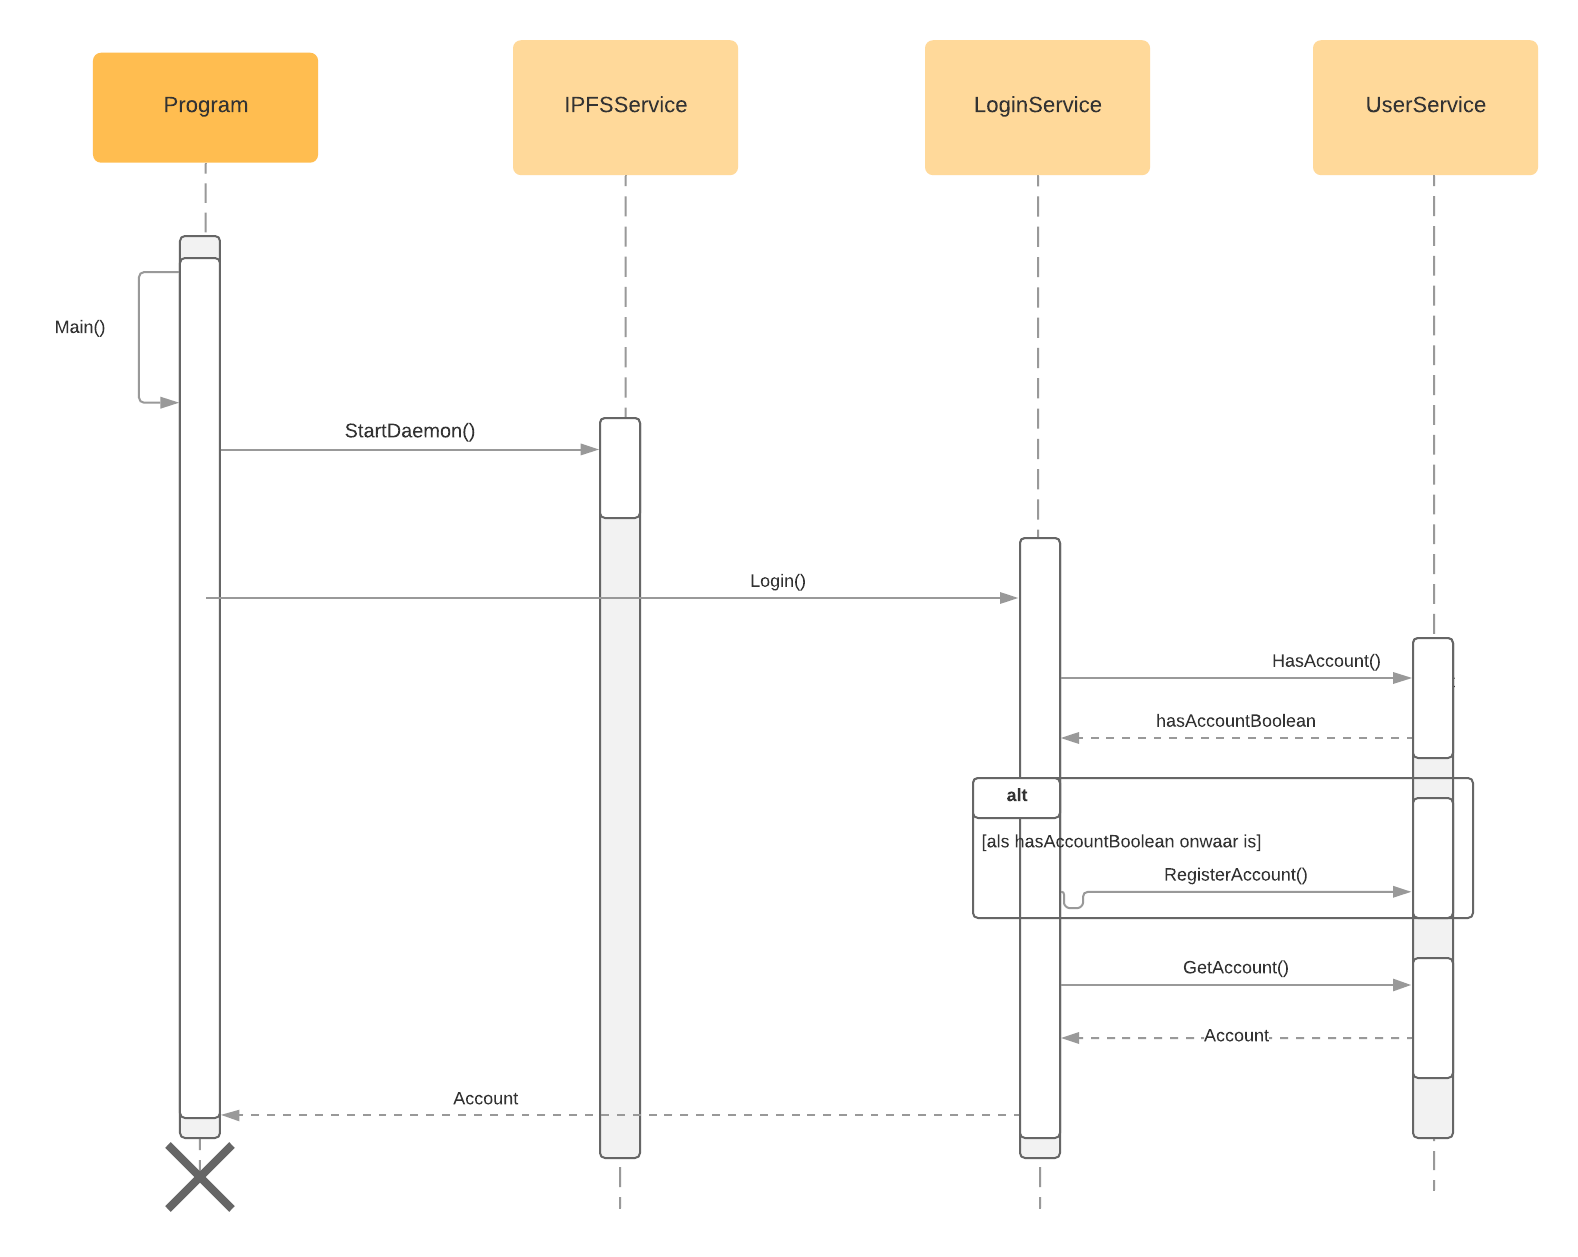
\includegraphics[scale=.4]{POC-1.png}
\caption[POC opstart]{Een sequentie diagram die de noodzakelijke opstart stappen overloopt. }
\end{figure}

\subsection{Het opslaan en opvragen van bestanden.}
Voor het opslaan en bijhouden van de bestanden wordt gebruik gemaakt van het concept van een Repository. Een repository zoals gedefineerd in deze bachelorproef is vergelijkbaar met het concept van een archief -zie \ref{}-. Het bevat een unieke naam, alle versies van bestanden 

\subsection{Het delen van bestanden met anderen}

\subsection{Het aanbrengen en binnenhalen van wijzigingen}

\subsection{Het teruggaan naar eerder versies}

Om de verschillende smartcontracts te ontwikkelen is er gekozen om gebruik te maken van een klasse diagram. Dit diagram biedt een schematisch overzicht van de verschillende contracten die ontwikkeld zijn alsook de verschillende functies en attributen

\textbf{TODO: Hier komt nog een klasse diagram alsook een kort overzicht van de oplossing}